\PassOptionsToPackage{table, dvipsnames}{xcolor}
\documentclass[a4paper,twoside,12pt]{toptesi}
\usepackage[T1]{fontenc}
\usepackage[utf8]{inputenc}
\usepackage[italian]{babel}
\usepackage{graphicx}
\usepackage{tikz}
\usetikzlibrary{positioning}
\usepackage{pgfplots}
\usepackage[font=small,skip=1pt]{caption}
\usepackage{xcolor}
\captionsetup[listing]{position=top}
\usepackage{subcaption}

%This equals 1.5 linespacing in Word
\linespread{1.25}

\let\savedlisting\listing
\AtBeginDocument{\let\listing\savedlisting}
\usepackage{listings}
\lstset{
  basicstyle=\ttfamily\footnotesize,
  keywordstyle= \ttfamily\footnotesize
}

\usepackage{bm}


\def\dept{DIPARTIMENTO DI INFORMATICA}
\def\course{CORSO DI LAUREA IN INFORMATICA}
\def\title{Sviluppo e Gestione di Chatbot Addestrati con Tecnica RAG tramite Servizi RESTful}
\def\author{Federico Calò}
\def\relatoreone{Prof.ssa  Berardina Nadja DE CAROLIS}
\def\relatoretwo{}
\def\subject{SISTEMI AD AGENTI}
\def\annoacc{2023 - 2024}
\def\beforecandidate{LAUREANDO:}
\def\beforetitle{TESI DI LAUREA \\ IN \\}
\def\beforeprof{RELATORI:}
\def\beforecorrelatore{CORRELATORI:}
\def\beforeannoacc{ANNO ACCADEMICO}

\makeatletter
\def\cleardoublepage{\clearpage\if@twoside \ifodd\c@page\else
    \hbox{}
    \vspace*{\fill}
    \vspace{\fill}
    \thispagestyle{empty}
    \newpage
    \if@twocolumn\hbox{}\newpage\fi\fi\fi}
\makeatother

\definecolor{codegreen}{rgb}{0,0.6,0}
\definecolor{codegray}{rgb}{0.5,0.5,0.5}
\definecolor{codepurple}{rgb}{0.19, 0.55, 0.91}
\definecolor{backcolour}{rgb}{1.0, 0.98, 0.98}

\lstdefinestyle{mystyle}{
    backgroundcolor=\color{backcolour},   
    commentstyle=\color{codegreen},
    keywordstyle=\color{codepurple},
    numberstyle=\tiny\color{codegray},
    stringstyle=\color{codepurple},
    basicstyle=\ttfamily\footnotesize,
    breakatwhitespace=false,         
    breaklines=true,                 
    captionpos=b,                    
    keepspaces=true,                 
    numbers=left,                    
    numbersep=5pt,                  
    showspaces=false,                
    showstringspaces=false,
    showtabs=false,                  
    tabsize=2
}
\lstset{style=mystyle}
\setlength{\parindent}{0pt}
\setlength{\parskip}{5pt}
\usepackage{hyperref}
\hypersetup{
    colorlinks = true,
    allcolors=black
}

\newcommand{\boldtt}[1]{\textbf{\texttt{#1}}}

\begin{document}

\begin{titlepage}
	\begin{tikzpicture}[remember picture,overlay]
		\centering
		\node[yshift=-6 cm] (logo) at (current page.north) {
\includegraphics[width=0.75\linewidth]{immagini/uniba.jpg}};
			\node[text width=50em,yshift=0.25cm, align = center, below = of logo](dipartimento){\normalsize \dept};
			\node[text width=40em, align = center, yshift=.55cm,below = of dipartimento](course){\normalsize \course};
		\node[text width=35em,align = center,  yshift=1.2cm,below = of course](line){\par\noindent\rule{\textwidth}{0.4pt}};
		\node[text width=40em, align = center, yshift=.55cm,below = of line](lia){\normalsize \beforetitle \xspace \subject };
		
  \node[text width=40em, align = center, yshift=-0.5cm,below = of lia](title){\bfseries \parbox{12cm}{\fontsize{21pt}{20pt}\selectfont \centering \title\par}};
  
	\node[text width=35em, align = left, yshift=-1cm,below = of title](relatoretit){\normalsize \textbf{\beforeprof} };
 	\node[text width=35em, align = left, yshift=1cm,below = of relatoretit](relatore){\large \relatoreone \\ \relatoretwo};


      
		\node[text width=35em, align = right, yshift=-1cm,below = of title](candidatetit){\normalsize \textbf{\beforecandidate}};
		 \node[text width=35em, align = right, yshift=1cm,below = of candidatetit](candidate){\large \author};


  \node[text width=35em,align = center,  yshift= -3cm,below = of candidate](line2){\par\noindent\rule{\textwidth}{0.4pt}};
	
  
  \node[text width=50em, align = center, yshift=0.5cm,below = of line2](year){\large \beforeannoacc\xspace \annoacc};
	\end{tikzpicture}
\end{titlepage}


\cleardoublepage


\pagenumbering{roman}

\tableofcontents

\cleardoublepage

\pagenumbering{arabic}
\setcounter{page}{1}
%\addcontentsline{toc}{chapter}{Introduzione}

\chapter{Introduzione}
Nel contesto attuale, caratterizzato da una crescente interazione tra utenti e sistemi digitali, i chatbot stanno emergendo come strumenti essenziali per migliorare l’esperienza dell’utente e ottimizzare i processi aziendali. Diverse ricerche evidenziano come l’adozione di chatbot possa ridurre significativamente i costi operativi, aumentare l’efficienza del servizio clienti e migliorare il tasso di soddisfazione degli utenti. Ad esempio, uno studio condotto da Gartner nel 2023 stima che entro il 2026 i chatbot contribuiranno a ridurre i costi aziendali del 30\%, sostituendo fino al 70\% delle interazioni umane in determinati contesti di servizio clienti. Inoltre, un rapporto di McKinsey sottolinea come le aziende che integrano chatbot nei propri processi abbiano registrato un aumento medio del 25\% nella velocità di risoluzione delle richieste.

Tuttavia, i chatbot tradizionali presentano alcune limitazioni significative, in particolare la mancanza di contesto nelle risposte fornite. Questi sistemi spesso si basano su algoritmi deterministici o su modelli di machine learning addestrati su dataset limitati, che non sono in grado di adattarsi dinamicamente a richieste complesse o ambigue. Ad esempio, un chatbot tradizionale potrebbe fornire risposte errate o incomplete in scenari in cui l’utente utilizza un linguaggio non strutturato, si riferisce a informazioni specifiche o richiede dati aggiornati in tempo reale. Tali limitazioni riducono la loro efficacia in applicazioni aziendali critiche, come l’assistenza tecnica avanzata o la consulenza personalizzata.

Per superare queste limitazioni, è stata adottata la metodologia Retrieval-Augmented Generation (RAG), che combina tecniche di recupero di informazioni (retrieval) e generazione di risposte (generation). L’approccio RAG consente ai chatbot di consultare un database di conoscenze esterno per reperire informazioni pertinenti e integrarle nella generazione di risposte, migliorando significativamente la pertinenza e la precisione delle interazioni. Ad esempio, un chatbot basato su RAG può accedere a documentazione tecnica, manuali aziendali o dati di mercato aggiornati, fornendo risposte dettagliate e contestualizzate anche a domande complesse.

Questa tesi si propone di affrontare la sfida della creazione e gestione di chatbot avanzati attraverso la progettazione e realizzazione di un ecosistema completo basato su RAG. L’obiettivo principale del progetto è sviluppare una piattaforma che consenta la creazione di diversi chatbot addestrati con questa metodologia, in grado di interfacciarsi tra loro e con l’utente attraverso servizi REST.

Per garantire una fruizione ottimale e una gestione efficiente dei chatbot, è stata progettata una soluzione integrata che comprende:
\begin{itemize}

\item \textbf{Servizi REST}: Interfacce di programmazione che permettono la comunicazione tra il frontend, i servizi backend e i vari bot. Le API sono state sviluppate utilizzando due tecnologie complementari: Spring Boot e Python.

\item \textbf{Bot RAG}: L'approccio Retrieval-Augmented Generation è stato adottato per addestrare i chatbot, sviluppati in Python, combinando tecniche di recupero di informazioni e generazione di risposte, al fine di migliorare la pertinenza e l'accuratezza delle risposte fornite dai bot.
\end{itemize}

La realizzazione di questo ecosistema richiede un'integrazione armoniosa di componenti software e tecniche di machine learning, mirata a offrire una piattaforma versatile e potente per lo sviluppo di chatbot avanzati. L'importanza di questo progetto risiede nella sua capacità di semplificare la creazione e gestione di chatbot sofisticati, migliorando significativamente l'interazione uomo-macchina e offrendo soluzioni scalabili per diverse applicazioni aziendali e di consumo.

Diversi contesti possono beneficiare di quanto realizzato, tra cui il settore sanitario, che è stato scelto come esempio di applicazione pratica durante il progetto. In questo ambito, i chatbot basati su RAG possono supportare il personale medico rispondendo a domande sui protocolli clinici, fornendo informazioni sui farmaci o assistendo i pazienti nella gestione delle loro cure.

Per quanto riguarda gli sviluppi futuri, questa tecnologia potrebbe evolversi integrando funzionalità di intelligenza artificiale più avanzate, come modelli di linguaggio di nuova generazione e algoritmi di apprendimento rinforzato. Tali innovazioni permetterebbero ai chatbot di adattarsi in tempo reale alle esigenze degli utenti, prevedere domande basandosi sul contesto e fornire un supporto ancora più personalizzato e proattivo.

Un'importante direzione di sviluppo potrebbe essere l'adozione della tecnica CAG (Cache-Augmented Generation), che combina l'uso di cache per memorizzare e riutilizzare risposte o conoscenze rilevanti. Grazie a questa tecnica, i chatbot sarebbero in grado di accedere rapidamente a informazioni precedenti, riducendo i tempi di elaborazione e migliorando la coerenza delle interazioni. La CAG consentirebbe inoltre ai bot di ottimizzare la gestione delle risorse computazionali, evitando calcoli ripetitivi per contenuti già generati e focalizzandosi sulle nuove richieste.

Inoltre, l'introduzione di una memoria a lungo termine rappresenterebbe una svolta significativa. Una memoria strutturata e persistente permetterebbe ai chatbot di ricordare dettagli e preferenze degli utenti nel tempo, garantendo interazioni coerenti e altamente personalizzate.

Infine, l'integrazione con sistemi IoT e dispositivi indossabili potrebbe ampliare ulteriormente le applicazioni, consentendo ai chatbot di raccogliere e analizzare dati in tempo reale. Questo approccio non solo migliorerebbe la precisione delle risposte, ma favorirebbe anche la creazione di servizi personalizzati ed efficaci, capaci di anticipare le esigenze degli utenti in contesti diversi.

\chapter{Large Language Models (LLM) e Retrieval-Augmented Generation (RAG)}
Nel contesto dell'intelligenza artificiale e del Natural Language Processing (NLP), i Large Language Models (LLM) e la metodologia Retrieval-Augmented Generation (RAG) rappresentano due pilastri fondamentali. Questo capitolo analizza l'evoluzione degli LLM, partendo dagli approcci simbolici iniziali fino agli avanzamenti moderni resi possibili dall'architettura Transformer. Successivamente, vengono approfondite le caratteristiche tecniche degli LLM, le loro applicazioni in diversi ambiti e le limitazioni che ne influenzano l'adozione. Inoltre, viene descritta la metodologia RAG, evidenziandone il funzionamento come combinazione tra generazione di contenuti e recupero di informazioni esterne, con particolare attenzione ai benefici, alle sfide e alle prospettive di sviluppo. Infine, si affrontano le implicazioni etiche e le potenziali direzioni future di queste tecnologie.

\section{Breve Storia e Evoluzione dei LLM}

I Large Language Models (LLMs) sono modelli avanzati di intelligenza artificiale progettati per comprendere, generare e interagire con il linguaggio umano a livelli di complessità senza precedenti, rappresentando l'apice dell'evoluzione dell'Intelligenza Artificiale (IA) e del Natural Language Processing (NLP).

L'evoluzione degli LLM segue un percorso che affonda le radici negli anni '50, quando l'intelligenza artificiale era ancora agli inizi, con sistemi basati su regole simboliche che analizzavano il linguaggio tramite regole sintattiche prestabilite. Tuttavia, questi modelli erano limitati dalla rigidità, incapaci di adattarsi a contesti o dati non previsti.

Negli anni '80 e '90, l'introduzione del machine learning e dei modelli statistici ha portato a un significativo passo avanti, con tecniche come gli n-grammi e i modelli di Markov nascosti che permettevano una gestione probabilistica del linguaggio. Sebbene abbiano superato alcune limitazioni dei sistemi simbolici, restava una mancanza di comprensione semantica profonda del contesto linguistico.

Con l'avvento delle reti neurali e del deep learning nei primi anni 2000, l'elaborazione del linguaggio naturale ha subito una trasformazione radicale. Le architetture come le reti neurali ricorrenti (RNN) e le Long Short-Term Memory (LSTM) hanno introdotto la capacità di gestire le dipendenze temporali e sequenziali, migliorando così l'efficacia dei modelli nella comprensione del testo.

La vera rivoluzione è avvenuta nel 2017 con la pubblicazione del paper "Attention is All You Need" di Vaswani et al., che ha introdotto l'architettura Transformer. Questo modello ha superato le limitazioni delle RNN, consentendo di analizzare l'intero contesto di un testo grazie al meccanismo di attenzione multi-head. L'architettura Transformer è diventata la base per modelli come GPT, BERT e T5, che hanno segnato una vera svolta nell'elaborazione del linguaggio naturale.

Oggi, modelli come GPT-3 e GPT-4 di OpenAI, con miliardi di parametri, rappresentano l'apice dell'evoluzione degli LLM, in grado di generare testi coerenti, tradurre lingue, scrivere codice e rispondere a domande complesse. Altri modelli, come BERT e T5, sono stati progettati per applicazioni specifiche, come la comprensione del contesto bidirezionale e la risoluzione di compiti NLP multi-task. In questo modo, gli LLM continuano a spingere i limiti di ciò che è possibile fare con il linguaggio naturale.

\section{Caratteristiche Fondamentali degli LLM}

Gli LLM si distinguono per la loro capacità di apprendere e rappresentare il linguaggio naturale in maniera sofisticata. Le loro caratteristiche principali includono:
\begin{itemize}
\item Addestramento su larga scala
\item Architettura Transformer
\item Rappresentazione vettoriale del testo
\end{itemize}

Gli LLM vengono addestrati su vasti dataset che comprendono miliardi di parole provenienti da fonti diversificate, come libri, articoli scientifici, siti web e conversazioni online. Questo approccio consente loro di apprendere relazioni semantiche complesse, nonché di generalizzare conoscenze anche in contesti che non sono stati direttamente inclusi durante l'addestramento. La forza dei Transformer risiede nell'architettura encoder-decoder e nei meccanismi di attenzione multi-head, che permettono di assegnare un peso maggiore a parole o frasi rilevanti all'interno di un contesto, ottimizzando così l'elaborazione delle informazioni. Questo meccanismo è fondamentale per gestire efficacemente le dipendenze a lungo termine nei testi, un compito che sarebbe difficile da affrontare con approcci precedenti.

Un altro aspetto cruciale negli LLM è la tokenizzazione, ovvero il processo che suddivide il testo in unità più piccole, dette token. Algoritmi come Byte Pair Encoding (BPE) o WordPiece vengono utilizzati per questa operazione, permettendo al modello di trattare in modo efficiente anche dati complessi. Successivamente, questi token vengono trasformati in vettori numerici che rappresentano le relazioni semantiche tra le parole, facilitando così la comprensione e la generazione di linguaggio naturale in modo coerente e contestuale.

\section{Applicazioni degli LLM}
I Large Language Models (LLMs) hanno trasformato radicalmente il campo dell'intelligenza artificiale e dell'elaborazione del linguaggio naturale (NLP), aprendo nuove opportunità applicative in vari settori. Grazie alla loro capacità di comprendere e generare testo con una precisione senza precedenti, sono diventati strumenti essenziali in numerosi ambiti.

Una delle applicazioni principali degli LLM è nei sistemi di assistenza virtuale. Tecnologie come Siri, Alexa e Google Assistant sfruttano gli LLM per interpretare il linguaggio naturale, comprendere il contesto e rispondere alle richieste degli utenti, eseguire comandi vocali, fornire informazioni in tempo reale e interagire con altre applicazioni, offrendo un'interazione fluida e naturale.

Nel settore della generazione di contenuti, gli LLM vengono utilizzati per produrre testi automaticamente, come articoli di notizie, post sui social media, descrizioni di prodotti e persino opere creative come poesie o storie. Modelli come GPT-3 sono in grado di generare contenuti di alta qualità, quasi indistinguibili da quelli scritti da esseri umani, rendendo la creazione di contenuti più veloce ed accessibile.

Gli LLM trovano anche ampio impiego nei sistemi di traduzione automatica. Servizi come Google Translate utilizzano questi modelli per tradurre testi da una lingua all'altra con una precisione crescente, grazie alla loro capacità di comprendere strutture linguistiche e relazioni semantiche, producendo traduzioni che rispettano il contesto e il significato originale.

Nel campo dell'analisi del sentiment e del monitoraggio dei social media, gli LLM vengono utilizzati per analizzare grandi volumi di dati testuali, come post sui social media, recensioni e articoli di opinione. Questa analisi consente alle aziende di comprendere l'opinione pubblica e monitorare il sentiment riguardo a prodotti, marchi o eventi, supportando decisioni strategiche basate sui feedback raccolti.

Un'altra applicazione emergente degli LLM è nel supporto alla scrittura e alla ricerca. Strumenti come quelli sviluppati da OpenAI assistono scrittori, ricercatori e studenti nella creazione di bozze, nel riassumere articoli, nel generare idee o nel formulare risposte a domande complesse. Questi modelli accelerano il processo creativo, migliorando la produttività e fornendo suggerimenti pertinenti in tempo reale.

Infine, gli LLM sono utilizzati nel supporto decisionale aziendale. Analizzando dati testuali e documenti, questi modelli aiutano le aziende a estrarre informazioni critiche, fare previsioni basate su tendenze emergenti e prendere decisioni strategiche, con applicazioni particolarmente utili in ambiti come l'analisi di mercato, la gestione del rischio e la pianificazione aziendale.

\section{Introduzione alla Retrieval-Augmented Generation (RAG)}
La metodologia Retrieval-Augmented Generation (RAG) è una tecnica avanzata che combina le capacità generative degli LLM con il recupero di informazioni da fonti esterne. RAG è stata introdotta da Facebook AI Research (FAIR) nel 2020 come risposta alle limitazioni degli LLM tradizionali. Questa tecnica integra un sistema di recupero (retrieval) con un modello generativo per:

\begin{itemize}
\item Garantire risposte contestuali e aggiornate.
\item Superare le limitazioni dei dati statici di addestramento degli LLM.
\end{itemize}

Il processo si divide in tre fasi:
\begin{itemize}
\item Recupero: Il modello cerca documenti rilevanti in un database esterno.
\item Fusione: Le informazioni recuperate vengono integrate nel contesto della domanda.
\item Generazione: L'LLM genera una risposta articolata basata sul contesto arricchito.
\end{itemize}

La metodologia rag può essere applicata in svariati contesti quali la creazione di chatbot avanzati i quali rispondono a domande tecniche o forniscono supporto personalizzato in settori come il customer service, oppure fornendo informazioni cliniche aggiornate basandosi su database di articoli scientifici, o infine può essere utilizzata per offrire supporto legale nella consultazione di alcuni documenti complessi.

Tra i vantaggi di questa metodologia troviamo l'aggiornabilità, in quanto si può accedere a dati aggiornati, superando in tal modo i limiti dei modelli pre-addestrati, un'elevata contestualizzazione, in quanto le risposte generate sono specifiche e rilevanti per il contesto dell'utente, e infine una precisione nelle risposte che vengono fornite all'utente.

\chapter{Analisi e progettazione}

Negli ultimi due decenni, i servizi RESTful (Representational State Transfer) hanno trasformato il modo in cui le applicazioni comunicano, emergendo come lo standard de facto per la progettazione di API scalabili e interoperabili. L'architettura REST, introdotta da Roy Fielding nella sua tesi di dottorato nel 2000, si basa su principi che enfatizzano la semplicità, l'indipendenza tecnologica e l'uso efficiente delle risorse di rete. La sua adozione su vasta scala ha facilitato l'interoperabilità tra sistemi eterogenei, rendendola un pilastro fondamentale dello sviluppo software moderno.

Un aspetto chiave del successo di REST è la sua natura stateless, che elimina la necessità per il server di mantenere lo stato delle richieste precedenti. Ogni richiesta HTTP include tutte le informazioni necessarie per essere processata, garantendo una maggiore scalabilità e semplificando l'architettura. Questo approccio consente ai servizi RESTful di gestire un elevato volume di richieste simultanee, un requisito essenziale per le moderne applicazioni distribuite.

La separazione tra client e server è un altro principio cardine di REST. Questo modello architettonico consente uno sviluppo modulare, in cui il frontend e il backend possono evolversi indipendentemente. Ad esempio, un'applicazione mobile può utilizzare le stesse API RESTful di un'applicazione web, garantendo una maggiore riusabilità del codice e riducendo i costi di manutenzione.

La storia dei servizi RESTful è strettamente legata alla crescita di Internet e delle applicazioni web. Negli anni '90, la necessità di una comunicazione efficiente tra sistemi in rete ha portato allo sviluppo di vari protocolli e architetture, ma molti di essi, come SOAP (Simple Object Access Protocol), risultavano troppo complessi o rigidi per soddisfare le esigenze in rapida evoluzione delle applicazioni moderne.

L'introduzione di REST ha segnato un cambiamento radicale, grazie alla sua enfasi sulla semplicità e sull'utilizzo di standard esistenti come HTTP. La sua adozione è stata accelerata dall'ascesa di applicazioni basate su microservizi, dove l'indipendenza e la modularità dei componenti erano requisiti fondamentali. Studi recenti, come quello di Richardson e Ruby nel libro "RESTful Web Services", sottolineano come REST abbia permesso di superare le limitazioni delle architetture precedenti, offrendo una soluzione flessibile e scalabile per la progettazione di API.

Con l'emergere dei modelli di linguaggio di grandi dimensioni (LLMs), come GPT e BERT, i servizi RESTful hanno trovato una nuova dimensione di applicazione. L'integrazione tra REST e LLMs consente di sfruttare le capacità avanzate di elaborazione del linguaggio naturale all'interno di architetture distribuite, creando un'infrastruttura potente e flessibile per applicazioni basate sull'intelligenza artificiale.

In questo progetto, i servizi RESTful fungono da intermediari tra i modelli LLMs, i database e le applicazioni client. La tecnica Retrieval-Augmented Generation (RAG), utilizzata per arricchire le risposte dei chatbot con dati specifici e aggiornati, si basa su questo approccio. Ad esempio, una richiesta HTTP proveniente da un client può attivare il recupero di informazioni da un database, che vengono poi elaborate da un modello LLM per generare una risposta contestualizzata e pertinente.

\section{Architettura del Sistema}

Il progetto adotta un'architettura basata su microservizi, implementata con Spring Boot per il backend e Python per l'addestramento e l'interrogazione dei modelli di linguaggio. Questa scelta tecnologica consente di sfruttare i punti di forza di ciascuna piattaforma: Spring Boot per la robustezza e la scalabilità delle API REST, e Python per la sua vasta gamma di librerie dedicate al machine learning e al Natural Language Processing.

Ogni microservizio è progettato per svolgere una funzione specifica, come l'autenticazione, la gestione delle richieste o l'elaborazione dei dati. Questo approccio modulare facilita l'estensibilità del sistema, permettendo di aggiungere nuovi chatbot o funzionalità senza compromettere l'infrastruttura esistente. I servizi RESTful, grazie alla loro natura indipendente dalla piattaforma, orchestrano la comunicazione tra i vari componenti del sistema, garantendo coerenza e flessibilità.

Un esempio pratico di applicazione è rappresentato dall'ambito sanitario. Ogni reparto di una struttura medica potrebbe disporre di un chatbot addestrato su documenti specifici, come protocolli clinici o linee guida. I chatbot, accessibili tramite un'interfaccia grafica condivisa, consentirebbero ai medici di consultare rapidamente informazioni pertinenti, migliorando la collaborazione interdisciplinare e l'efficienza operativa.

L'integrazione tra i servizi REST e i modelli LLMs offre molteplici vantaggi:

Uno degli aspetti più significativi dell'uso di REST in combinazione con gli LLMs è la capacità di fornire esperienze personalizzate. Analizzando le richieste degli utenti, i sistemi possono adattare le risposte ai bisogni specifici, migliorando non solo la soddisfazione dell'utente ma anche l'efficacia delle interazioni. Questo approccio personalizzato è particolarmente utile in contesti come il customer service, dove è cruciale rispondere rapidamente e accuratamente a un'ampia varietà di richieste.

Inoltre, la natura stateless di REST garantisce interazioni robuste, minimizzando il rischio di errori legati a sessioni instabili o a interruzioni nella comunicazione. Questo aspetto è particolarmente rilevante in applicazioni mission-critical, come quelle mediche o finanziarie, dove l'affidabilità è essenziale. L'architettura REST, combinata con le capacità degli LLMs, consente di bilanciare richieste ad alta intensità computazionale, garantendo prestazioni fluide anche in situazioni di carico elevato.

Un altro vantaggio significativo è rappresentato dalla scalabilità. I sistemi distribuiti basati su REST possono essere facilmente estesi per gestire un numero crescente di richieste, rendendo questa combinazione ideale per applicazioni globali che operano in ambienti multilingue e multi-dominio. Ad esempio, i chatbot possono fornire risposte in diverse lingue, accedendo a fonti di informazione localizzate e garantendo un'esperienza uniforme agli utenti di tutto il mondo.

Un caso emblematico di miglioramento dell'esperienza utente attraverso REST e LLMs è l'implementazione di sistemi di assistenza virtuale in tempo reale. In questi scenari, i chatbot possono integrare informazioni provenienti da database esterni e modelli predittivi per fornire risposte contestuali e aggiornate. L'uso del caching, inoltre, riduce i tempi di latenza, migliorando ulteriormente l'interazione utente-macchina.

Infine, l'adattabilità di questa combinazione è fondamentale per supportare applicazioni in costante evoluzione. Gli sviluppatori possono aggiornare i modelli di linguaggio o modificare le API REST senza interrompere il servizio, garantendo così un ciclo di sviluppo continuo e una rapida risposta alle nuove esigenze degli utenti.

Il capitolo "Analisi e progettazione" approfondisce i legami tra i servizi RESTful e i modelli di linguaggio avanzati, evidenziando come questa combinazione rappresenti una soluzione potente per lo sviluppo di applicazioni moderne. Attraverso un'analisi dettagliata delle scelte tecnologiche e dell'architettura implementata, si dimostra come i principi di REST possano essere sfruttati per creare sistemi scalabili, modulari e altamente efficienti. Questo approccio non solo soddisfa le esigenze attuali, ma offre anche una solida base per futuri sviluppi tecnologici.

\section{Applicazione}

Per testare la fattibilità di integrare chatbot addestrati con la metodologia RAG (Retrieval-Augmented Generation) in un sistema complesso basato su microservizi e chiamate REST, è stato scelto come caso di studio l'ambito sanitario. In particolare, si è sviluppato un sistema per la gestione dei pazienti che include un chatbot addestrato su alcune schede dietetiche tratte dal progetto SISTER. Quest'ultimo progetto, incentrato sull'invecchiamento attivo degli anziani, ha dedicato particolare attenzione alle diete personalizzate come strumento per prevenire la fragilità biopsicosociale, dimostrando come un approccio multidisciplinare possa migliorare la qualità della vita attraverso interventi mirati e basati su evidenze scientifiche.




Si sono creati diversi microservizi in SpringBoot:
\begin{itemize}
\item bff
\item bot alimentazione
\item ms infermiere
\item ms medico
\item ms pazienti
\item system management
\end{itemize}

Il BFF rappresenta lo strato di comunicazione tra i microservizi e l'interfaccia di frontend, fungendo da intermediario per gestire le richieste e restituire i dati in modo ottimale. Il progetto Bot Alimentazione è dedicato alla gestione del chatbot addestrato sulle schede dietetiche, fornendo risposte personalizzate e basate sui dati nutrizionali. Il microservizio MS Infermiere si occupa della gestione degli infermieri e delle loro attività operative, mentre MS Medico è responsabile delle funzionalità legate ai medici, come la gestione delle consultazioni e delle prescrizioni. Allo stesso modo, MS Pazienti è focalizzato sulle operazioni riguardanti i pazienti, inclusi l'archiviazione dei dati clinici e il monitoraggio delle loro attività. Infine, il progetto System Management è stato progettato per gestire e addestrare i chatbot, garantendo un aggiornamento continuo delle funzionalità e un miglioramento costante delle prestazioni. Questa architettura modulare consente una chiara separazione delle responsabilità, assicurando flessibilità e scalabilità all’intero sistema.

I bot sviluppati in Python sono invece:
\begin{itemize}
\item bot alimentazione
\item bot sanitario
\end{itemize}

Il bot dedicato all'alimentazione comunica con il microservizio corrispondente, Bot Alimentazione, sviluppato in Spring Boot. Questo microservizio è addestrato utilizzando file PDF contenenti informazioni relative all'alimentazione, consentendo al bot di fornire risposte accurate e personalizzate in questo ambito. Il Bot Sanitario, invece, interagisce con i microservizi MS Infermiere, MS Medico e MS Pazienti. Questo bot può essere addestrato su materiale sanitario specifico, rendendolo uno strumento versatile e utile per medici, infermieri e pazienti, fornendo supporto in base alle esigenze di ciascun ruolo.

Tutti i microservizi interagiscono con un database progettato e implementato utilizzando SQL, che funge da archivio centrale per la gestione delle informazioni. Nel database vengono memorizzati i dati relativi all'addestramento dei bot, comprese le cartelle dei documenti caricati, insieme alle tabelle dedicate alla gestione delle sezioni riguardanti medici, infermieri e pazienti. Questo approccio garantisce una struttura organizzata e un accesso efficiente ai dati necessari per il funzionamento e l'evoluzione del sistema.
\\ \\ \\
Ogni bot si basa su queste tecnologie:

\begin{itemize}
\item Python
\item LangChain
\item Ollama
\end{itemize} 

Spring Boot è utilizzato per lo sviluppo dei servizi RESTful che costituiscono il cuore del backend del sistema. Questa potente piattaforma Java semplifica la creazione di applicazioni stand-alone e basate su microservizi. Spring Boot consente di costruire API REST robuste e scalabili, gestendo in modo efficiente le comunicazioni tra il frontend e i vari componenti del backend, e garantendo un'architettura modulare e facilmente estendibile.

Python, infine, è impiegato per la creazione e l'addestramento dei bot. Conosciuto per la sua sintassi chiara e la vasta gamma di librerie specializzate, Python è particolarmente adatto per il machine learning e l'elaborazione del linguaggio naturale. Le librerie di Python, come TensorFlow e PyTorch, permettono di sviluppare modelli avanzati per i bot, che possono essere addestrati per rispondere in modo preciso e contestuale alle esigenze degli utenti.

LangChain è un framework a supporto di Python per la vettorizzazione dei documenti sui quali si desidera addestrare il bot, per la tokenizzazione della domande dell'utente e il calcolo del coefficente di similarità tra la tokenizzazione della domanda e la tokenizzazione dei documenti. LangChain si coordina con Ollama, software per il download e l'avvio di LLM in locale.

La relazione tra queste tecnologie può essere rappresentata in modo chiaro ed efficace attraverso il seguente schema:
\begin{center}

\fbox{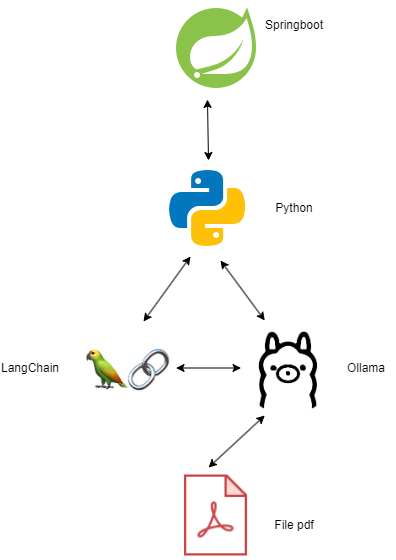
\includegraphics[width=0.42\textwidth, height=0.7\textheight, keepaspectratio]{immagini/3.png}}

\end{center}

Ollama permette di scaricare e utilizzare localmente il modello linguistico (LLM) desiderato, offrendo una soluzione che coniuga efficienza e sicurezza. Questa tecnologia consente di eseguire l'intero programma direttamente su un server locale, eliminando la necessità di trasferire dati sensibili verso piattaforme cloud esterne. Grazie a questa architettura, è possibile conservare i file PDF e altri dati critici in un ambiente controllato, riducendo al minimo i rischi di accessi non autorizzati o violazioni della privacy.

Oltre a garantire una maggiore protezione dei dati, l'approccio locale contribuisce a ridurre i costi operativi legati all'infrastruttura. L'assenza di dipendenze da servizi cloud esterni non solo abbatte i costi ricorrenti di archiviazione e calcolo, ma aumenta anche l'autonomia nella gestione del sistema, semplificando il controllo delle risorse hardware e software. Questa configurazione è particolarmente vantaggiosa per aziende e organizzazioni che devono trattare dati sensibili o rispettare rigorosi requisiti di conformità normativa.


\begin{center}

\fbox{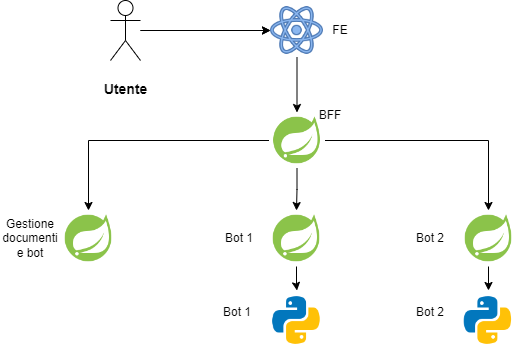
\includegraphics[width=0.8\textwidth, height=0.8\textheight, keepaspectratio]{immagini/2.png}}
\end{center}

In un'infrastruttura complessa composta da più bot che operano contemporaneamente, l'orchestrazione del sistema può essere organizzata in modo chiaro e modulare. Ciascun bot è costituito da due componenti principali: un progetto Python, che si occupa dell'addestramento e dell'interrogazione del modello linguistico (LLM) sui relativi file PDF, e un servizio Spring Boot, che funge da ponte per consentire al bot di comunicare con il resto dell'applicativo.

A supporto di questa struttura, esiste un progetto Spring Boot separato, dedicato alla gestione del caricamento dei documenti per ogni bot. Questo servizio è inoltre responsabile della registrazione dei bot nel database, garantendo un'integrazione coerente e centralizzata delle varie istanze operative.

Per completare l'infrastruttura, un ulteriore progetto Spring Boot è implementato come Backend For Frontend (BFF), che funge da intermediario tra un eventuale frontend e l'intero backend. Questa soluzione facilita le interazioni, offrendo un punto di accesso unico e semplificando la comunicazione tra le varie componenti del sistema.

Questa configurazione modulare non solo rende l'infrastruttura facilmente scalabile, consentendo l'aggiunta di nuovi bot, ma garantisce anche una gestione efficiente e una comunicazione fluida tra le diverse parti dell'ecosistema.

\subsection{Creazione e addestramento dei chatbot}

Nell'infrastruttura creata, ogni volta che è necessario sviluppare e addestrare un nuovo chatbot su documenti PDF specifici di una determinata tematica, viene creato un progetto in Python che utilizza quattro librerie chiave:

\begin{itemize}
	\item Flask: Questa libreria consente di creare endpoint REST, facilitando la comunicazione tra il chatbot e l'applicazione backend basata su Spring Boot tramite il protocollo REST.
	\item LangChain e Chroma: Queste librerie sono responsabili della vettorizzazione dei documenti PDF e del recupero delle informazioni rilevanti in risposta ai prompt inseriti dagli utenti attraverso l'interfaccia grafica.
	\item Ollama: Permette l'interazione tra il programma e il modello di LLM (Large Language Model) installato localmente, gestendo le richieste e le risposte del chatbot.
\end{itemize}

Parallelamente, viene avviato un progetto in Spring Boot per gestire la comunicazione tra il chatbot e l'interfaccia grafica tramite il protocollo REST, garantendo un'integrazione fluida e coerente tra il frontend e il backend.

\begin{lstlisting}[language=Python, caption=Microservizi Python]
@app.route('/message', methods=['POST'])
def botAlimentazioneMessage():
    jsonContent = request.json
    query = jsonContent.get('query')
    print(f"Query: {query}")

    response = llm.invoke(query)
    responseAnswer = {"message": check_and_translate(response)}

    return responseAnswer


@app.route('/load-pdf', methods=['POST'])
def loadPdf():
    file = request.files['file']
    fileName = file.filename
    saveFile = ""
    if os.name == 'nt':
        saveFile = pathAddestramento + "\\" + fileName
    else:
        saveFile = pathAddestramento + "/" + fileName
    file.save(saveFile)
    print(f"File salvato: {saveFile}")

    if not fileName[-4:] == ".pdf":
        response = {
            "status": "success",
            "fileName": fileName,
            "docLen": 0,
            "chunks": 0
        }
        return response

    loadPdf = PDFPlumberLoader(saveFile)

    docs = loadPdf.load_and_split()
    print(f"Doc len: {len(docs)}")

    chunks = text_splitter.split_documents(docs)
    print(f"Doc len: {len(chunks)}")

    response = {
        "status": "success",
        "fileName": fileName,
        "docLen": len(docs),
        "chunks": len(chunks)
    }
    if(len(docs)==0 or len(chunks)==0 ):
        response = {
            "status": "failed",
            "fileName": fileName,
            "docLen": len(docs),
            "chunks": len(chunks)
        }
    else:
        vectorStore = Chroma.from_documents(documents=chunks, embedding=embedding, persist_directory=pathAddestramento)
        vectorStore.persist()
    return response


@app.route('/message-pdf', methods=['POST'])
def askPdf():
    jsonContent = request.json
    query = jsonContent.get('query')
    print(f"Query: {query}")

    print(f"Carico il VectorStore")
    vectorStore = Chroma(persist_directory=pathAddestramento,
                         embedding_function=embedding)

    print(f"Creo la chain")
    retriever = vectorStore.as_retriever(
        search_type="similarity_score_threshold",
        search_kwargs={
            "k": 20,
            "score_threshold": 0.3,
        },
    )

    document_chain = create_stuff_documents_chain(llm, rawPrompt)
    chain = create_retrieval_chain(retriever, document_chain)

    result = chain.invoke({"input": f"Rispondi in italiano: {query}"})

    print(result)

    sources = []
    for doc in result["context"]:
        sources.append(
            {"source": doc.metadata["source"], "pageContent": doc.page_content}
        )

    responseAnswer = {"answer": check_and_translate(result["answer"]), "sources": sources}

    return responseAnswer


def startApplication():
    connessioneDb()
    recuperoPathAddestramento()
    app.run(host='127.0.0.1', port=5002, debug=True)
        
\end{lstlisting}

Ogni bot sarà collegato a una porta specifica e avrà tre endpoint in Python:

\begin{itemize}
\item "/load-pdf": per caricare il file e addestrare il bot sul file pdf
\item "/message": per dialogare con LLM non addestrato
\item "/message-pdf": per dialogare con LLM addestrato
\end{itemize}

Quando viene richiamato il path "/load-pdf", il file caricato viene tokenizzato e memorizzato all'interno del vectorstore. Successivamente, richiamando l'endpoint "/message-pdf", l'algoritmo tokenizza la domanda dell'utente e la confronta con i token dei file PDF già presenti nel vectorstore per fornire una risposta pertinente.

\newpage

\begin{lstlisting}[language=Java, caption=Microservizio Java]
@Operation(summary = "Chat normale",
            description = "Invio di un messaggio al bot Alimentazione sfruttando l'LLM non addestrato")
    @ApiResponses(value = {
            @ApiResponse(responseCode = "200", description = "Operazione andata a buon fine"),
            @ApiResponse(responseCode = "500", description = "Errore di sistema")
    })
    @GetMapping(value = "/normal-chat", produces = MediaType.APPLICATION_JSON_VALUE)
    public ResponseEntity<GenericResponseDto<String>> normalChat(@RequestParam String messagge) {
        return ResponseEntity.ok(esitoMessaggiRequestContextHolder.buildGenericResponse(chatService.normalChat(messagge)));
    }

    @Operation(summary = "Chat addestrata",
            description = "Invio di un messaggio al bot Alimentazione sfruttando l'LLM addestrato")
    @ApiResponses(value = {
            @ApiResponse(responseCode = "200", description = "Operazione andata a buon fine"),
            @ApiResponse(responseCode = "500", description = "Errore di sistema")
    })
    @GetMapping(value = "/chat-addestrata", produces = MediaType.APPLICATION_JSON_VALUE)
    public ResponseEntity<GenericResponseDto<ResponseMessagePdfDto>> chatAddestrata(@RequestParam String messagge) {
        return ResponseEntity.ok(esitoMessaggiRequestContextHolder.buildGenericResponse(chatService.chatAddestrata(messagge)));
    }
        
\end{lstlisting}

Nel corrispettivo progetto in Java, abbiamo i seguenti endpoint:
\begin{itemize}
\item "/normal-chat"
\item "/chat-addestrata"
\end{itemize}

Il primo endpoint consente di inviare un messaggio all'applicazione per ottenere una risposta generata da un modello di linguaggio non addestrato. Quando un utente invia un messaggio a questo endpoint, il sistema lo inoltra a un servizio Python che interroga il modello AI non personalizzato. La risposta generata viene quindi restituita all'utente in modo diretto, senza ulteriori informazioni di supporto. Il secondo endpoint, offre un'interazione più sofisticata. Anche in questo caso, l'utente fornisce un messaggio, ma il sistema lo inoltra a un servizio Python diverso, che interroga un modello di linguaggio addestrato su un insieme specifico di dati. Questo modello non solo genera una risposta, ma restituisce anche i file e le sezioni di contenuto utilizzate per formulare la risposta. Ciò consente all'utente di comprendere su quali informazioni il modello ha basato la sua elaborazione, rendendo questa opzione particolarmente utile per casi d'uso che richiedono maggiore trasparenza e tracciabilità.

Questi due endpoint rappresentano quindi due livelli distinti di interazione con i modelli di linguaggio: uno generico e immediato, l'altro personalizzato e più informativo.

\subsection{Progettazione del database}
Durante la fase di sviluppo è stato utilizzato un database relazionale, gestito tramite il linguaggio SQL, denominato botRag. Per configurare lo schema di base necessario al funzionamento dei microservizi, è sufficiente eseguire lo script creazioneTabelle.sql, che contiene tutte le query necessarie per la creazione delle tabelle. Questo script definisce la struttura del database, garantendo che tutti i microservizi possano accedere e manipolare i dati in modo corretto. 

L'URL di connessione al database utilizzato è: jdbc:mysql://localhost:3306/. Nel caso in cui la porta di connessione venga modificata o si decida di utilizzare un database in cloud, sarà necessario aggiornare il file di configurazione nei vari microservizi e nei progetti Python. Questo passaggio è fondamentale per garantire il corretto collegamento al database e il funzionamento del sistema.
\\

\fbox{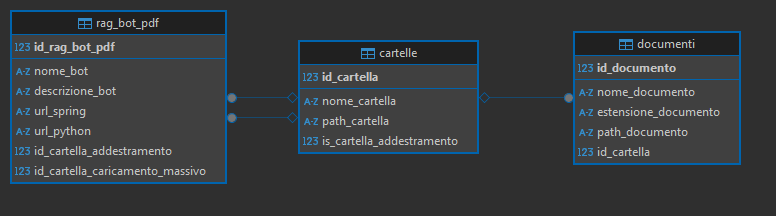
\includegraphics[width=0.8\textwidth, height=0.7\textheight, keepaspectratio]{immagini/Database bot.png}}

Il sistema di gestione dei dati per l'addestramento dei bot è organizzato secondo un modello relazionale composto da tre tabelle principali: \textbf{rag\scalebox{0.5}[1.0]{\_}bot\scalebox{0.5}[1.0]{\_}pdf}, \textbf{cartelle} e \textbf{documenti}. Di seguito viene descritto il ruolo e la struttura di ciascuna tabella, nonché le relazioni tra di esse. La tabella \textbf{rag\scalebox{0.5}[1.0]{\_}bot\scalebox{0.5}[1.0]{\_}pdf} contiene le configurazioni necessarie per ciascun bot. Qui di seguito vengono descritti i campi della tabella:

\begin{itemize}
\item \textbf{\textnormal{\lstinline|id_rag_bot_pdf|}}: Identificativo univoco del bot.
\item \textnormal{\lstinline|nome_bot|}: nome del bot
\item \textnormal{\lstinline|descrizione_bot|}: descrizione del bot
\item \textnormal{\lstinline|url_spring|}: URL utilizzato per l'integrazione con servizi esterni implementati in Spring.
\item \textnormal{\lstinline|url_python|}: URL utilizzato per l'integrazione con servizi esterni implementati in Python
\item \textnormal{\lstinline|id_cartella_addestramento|}: Riferimento alla cartella che contiene i file utilizzati per l'addestramento singolo del bot.
\item \textnormal{\lstinline|id_cartella_caricamento_massivo|}: Riferimento alla cartella utilizzata per la funzionalità di addestramento massivo.
\end{itemize}

La tabella \textbf{cartelle} è destinata alla gestione delle directory utilizzate per l'addestramento. Qui di seguito vengono descritti i campi della tabella:

\begin{itemize}
\item \textnormal{\lstinline|id_cartella|}: Identificativo univoco della cartella.
\item \textnormal{\lstinline|nome_cartella|}: Nome della cartella.
\item \textnormal{\lstinline|path_cartella|}: Percorso della cartella nel file system.
\item \textnormal{\lstinline|is_cartella_addestramento|}: Campo booleano che distingue tra:
	\begin{itemize}
	\item Cartella di addestramento singolo: Contiene i file già pronti per essere utilizzati nel processo di addestramento del bot.
	\item Cartella di addestramento massivo: Utilizzata esclusivamente per conservare file che verranno successivamente spostati nella cartella di addestramento singolo al 					momento dell’esecuzione della funzionalità di addestramento massivo.
	\end{itemize}
\end{itemize}

Il campo \textnormal{\lstinline|is_cartella_addestramento|} gioca un ruolo fondamentale nel distinguere le due tipologie di cartelle. La cartella di addestramento singolo è utilizzata direttamente nel processo di addestramento del bot, mentre la cartella di addestramento massivo funge da spazio temporaneo per conservare file che verranno successivamente caricati nella cartella di addestramento singolo. Questa distinzione consente di gestire in modo efficiente processi di addestramento su larga scala, garantendo la separazione tra i file temporanei e quelli effettivamente utilizzati dal bot.

La tabella documenti rappresenta i file utilizzati nel processo di addestramento. Qui di seguito vengono descritti i campi della tabella:
\begin{itemize}
\item \textnormal{\lstinline|id_documento|}: Identificativo univoco del documento.
\item \textnormal{\lstinline|nome_documento|}: Nome del file.
\item \textnormal{\lstinline|estensione_documento|}: Estensione o formato del file
\item \textnormal{\lstinline|path_documento|}: Percorso del file nel file system.
\item \textnormal{\lstinline|id_cartella|}: Collegamento alla cartella di appartenenza.
\end{itemize}

Le tre tabelle sono collegate per formare un sistema relazionale:
\begin{itemize}
\raggedright
\item La tabella \textnormal{\lstinline|rag_bot_pdf|} è associata alla tabella cartelle tramite i campi \textnormal{\lstinline|id_cartella_addestramento|} e \textnormal{\lstinline|id_cartella_caricamento_massivo|}, consentendo di associare un bot a due diverse directory: una per l'addestramento singolo e una per il caricamento massivo.
\item La tabella cartelle, a sua volta, è collegata alla tabella documenti tramite il campo \textnormal{\lstinline|id_cartella|}, che associa ogni documento a una specifica cartella.
\end{itemize}

Le altre tabelle del database sono destinate alla gestione del sistema sanitario in cui l'applicativo sarà utilizzato. Non fanno parte della gestione dei bot, ma possono essere adattate in base al contesto in cui i bot vengono creati. In futuro, si prevede comunque la possibilità di addestrare un bot utilizzando i dati presenti nel database e di sviluppare una memoria interna per il bot.

\subsection{Creazione dei microservizi REST}

Dopo aver creato i bot attraverso i relativi progetti in Python, come descritto nella sezione 2.1.1, si è proceduto allo sviluppo dei corrispondenti microservizi utilizzando Spring Boot, inclusa la realizzazione del microservizio System Management. I progetti relativi ai bot espongono endpoint specifici per consentire la comunicazione con gli altri componenti del sistema.

Il microservizio System Management adotta la metodologia Object-Relational Mapping (ORM) per mappare le entità del database su oggetti Java, agevolando la manipolazione dei dati e garantendo una stretta integrazione con la logica applicativa. Questo microservizio fornisce endpoint per operazioni essenziali come la registrazione, l'aggiornamento e l'eliminazione dei bot. Inoltre, include funzionalità per il caricamento dei file necessari e l'addestramento dei modelli, contribuendo a una gestione centralizzata ed efficace del ciclo di vita dei bot.

Un ruolo cruciale è svolto dal microservizio BFF (Backend for Frontend), progettato per fungere da ponte tra il front-end e gli altri microservizi. Al suo interno vengono memorizzati i file YAML, che descrivono le configurazioni e le specifiche di comunicazione tra i vari microservizi. Questo approccio semplifica il flusso dei dati, migliorando la modularità e riducendo la complessità nelle interazioni tra front-end e back-end. Il BFF consente al sistema di mantenere una chiara separazione delle responsabilità: i microservizi relativi ai bot e al System Management gestiscono rispettivamente le funzionalità core e la logica applicativa, mentre il BFF offre un'interfaccia ottimizzata per il front-end, migliorando l'esperienza utente e l'efficienza complessiva del sistema.

La configurazione dei path necessari per la comunicazione tra i microservizi è gestita dalla classe ExternalApiClientConfig, che centralizza e organizza i riferimenti ai percorsi esposti. Questo approccio garantisce una struttura modulare e facilmente manutenibile, permettendo di stabilire in modo chiaro e flessibile i percorsi per invocare le funzionalità offerte dai microservizi.

La gestione delle risposte derivanti dalle chiamate ai microservizi è affidata alla classe EsitoResponseErrorHandler, che si occupa di convertire e uniformare le risposte ricevute. Tali risposte vengono incapsulate in un oggetto generalizzato del tipo generico T, che include:

\begin{itemize}
\item un identificativo dell'operazione
\item una lista di messaggi che possono contenere informazioni, avvisi o errori,
\item il tipo di esito che specifica se l'operazione è andata a buon fine o meno.
\end{itemize}

Questa struttura consente una gestione uniforme delle risposte, migliorando la leggibilità e la manutenzione del codice. La generalizzazione introdotta dalla classe EsitoResponseErrorHandler offre inoltre maggiore flessibilità nel trattamento delle risposte, indipendentemente dal tipo specifico di payload restituito.

Nei microservizi REST progettati per interagire con i bot addestrati utilizzando la metodologia RAG (Retrieval-Augmented Generation), sono stati implementati controller che espongono endpoint specifici per gestire tre tipi principali di comunicazione: l'invio di messaggi alla chat non addestrata, l'interazione con la chat addestrata, e la generazione di risposte valutate secondo diverse metriche di qualità. Questa architettura garantisce un'integrazione modulare ed efficiente, permettendo ai sistemi di adattarsi dinamicamente alle richieste degli utenti e di ottimizzare l'elaborazione dei dati tramite metriche predefinite.

Per facilitare l'interazione con gli endpoint esposti dai microservizi, è stato integrato Swagger UI, un'interfaccia grafica intuitiva che permette agli sviluppatori e agli utenti di esplorare e testare gli endpoint. Swagger UI genera automaticamente documentazione interattiva basata su annotazioni presenti nel codice, rendendo l'accesso agli endpoint più immediato e agevole. Questa integrazione offre una soluzione user-friendly per inviare richieste e visualizzare risposte, eliminando la necessità di strumenti esterni o conoscenze approfondite dei dettagli di implementazione.

\chapter{Risultati}

In questo capitolo vengono presentati i risultati ottenuti durante l'implementazione del progetto, con un focus sull'interfaccia grafica realizzata tramite Swagger UI. Verranno illustrate le principali componenti sviluppate e verranno forniti esempi pratici di domande e risposte generate dal bot in risposta a specifiche richieste. L'analisi si concentra sull'efficacia delle funzionalità implementate e sull'esperienza utente offerta dalla piattaforma.

\section{Interfaccia del BFF}

Nel contesto dell’implementazione del BFF (Backend for Frontend), l’interfaccia Swagger UI consente di esporre in modo strutturato e intuitivo gli endpoint dei vari microservizi verso il front-end. Ogni endpoint è evidenziato con un colore specifico in base alla tipologia dell’operazione che rappresenta: verde per le operazioni di creazione (POST), azzurro per il recupero di informazioni (GET) e rosso per la rimozione di risorse (DELETE).

Gli endpoint sono organizzati in controller tematici, ciascuno dedicato a una specifica area funzionale del sistema. Ad esempio, il Gestione delle cartelle Controller è focalizzato sulla gestione delle directory dei bot, mentre il Gestione bot rag Controller si occupa delle operazioni di registrazione, modifica, ricerca e cancellazione dei bot, oltre alla gestione delle cartelle di addestramento. Questo approccio modulare consente di migliorare la chiarezza e l’efficienza del sistema, facilitando il recupero degli endpoint rilevanti per una determinata area di interesse.

La struttura organizzativa e l’utilizzo di colori distintivi rendono l’interfaccia Swagger UI uno strumento essenziale per interagire in modo efficace con il BFF, semplificando la comunicazione tra i microservizi e il front-end.

\fbox{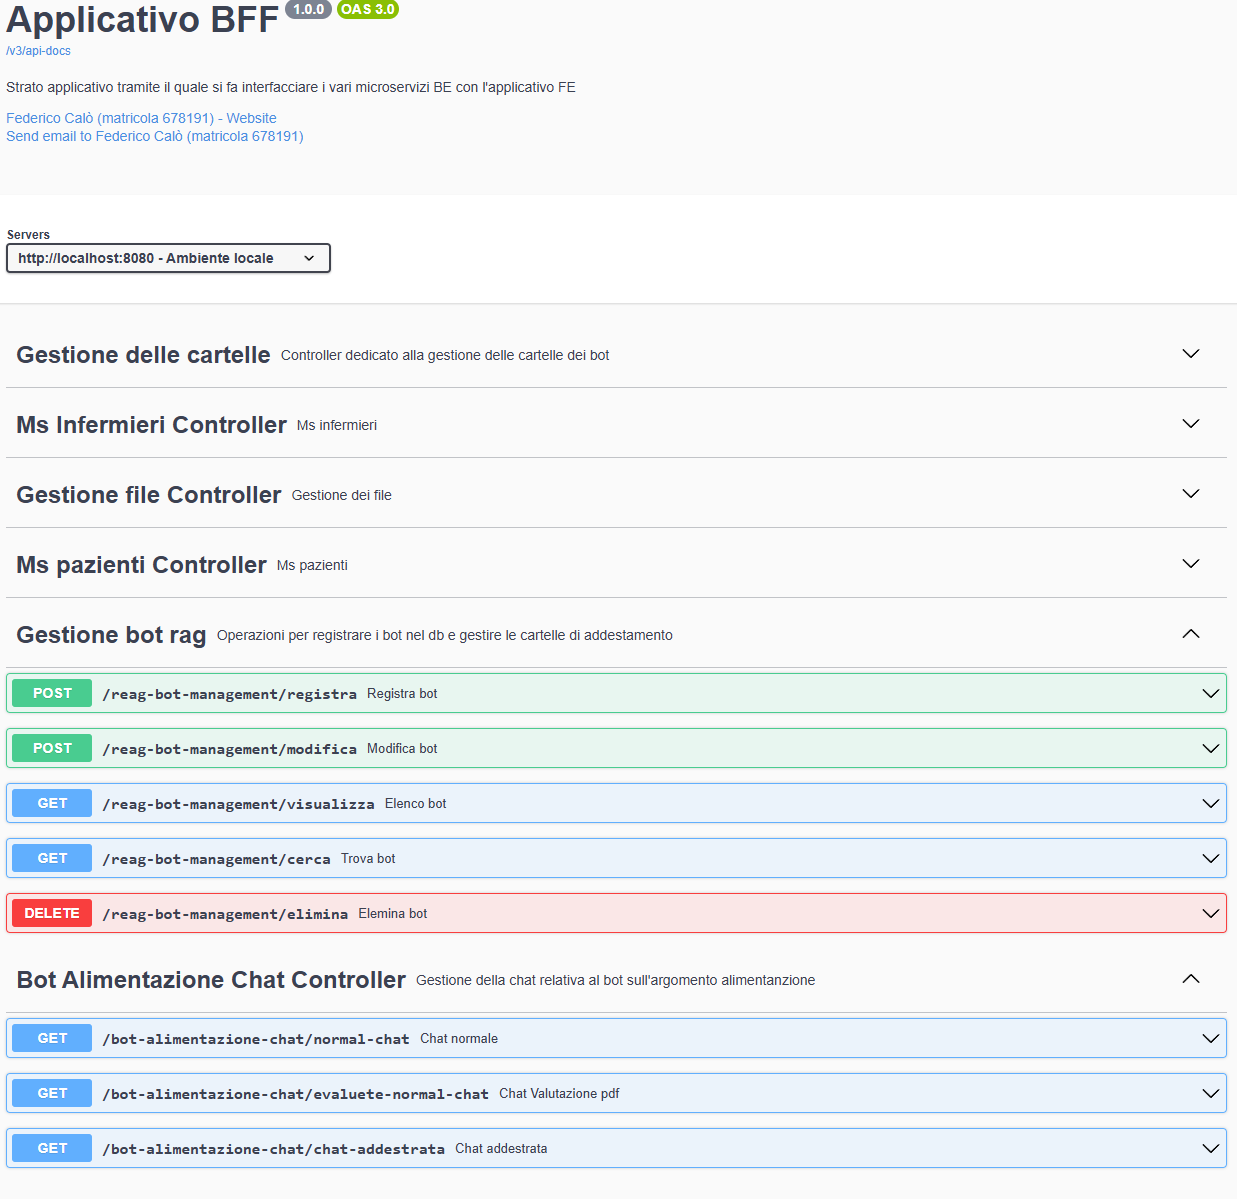
\includegraphics[width=0.9\textwidth, height=0.8\textheight, keepaspectratio]{immagini/bff.png}}

Ogni endpoint è strutturato in modo dettagliato per garantire una documentazione chiara e completa. Le chiamate sono definite dal path specifico, con eventuali parametri di query (path param) indicati, come nel caso del parametro obbligatorio message evidenziato nell'esempio. Per le operazioni che richiedono un payload, come le chiamate POST, viene previsto un oggetto nel corpo della richiesta (body).

La risposta è restituita in formato JSON, comprendendo informazioni dettagliate sullo stato dell'operazione. Nell’esempio riportato, per una chiamata andata a buon fine (200 - Operazione andata a buon fine), il JSON include un campo esito con i dettagli del codice di risposta, un messaggio esplicativo e i parametri associati. Inoltre, il payload restituito contiene informazioni come la query inviata, la similarità, i contenuti delle pagine e la fonte dei dati.

La gestione degli errori è anch’essa ben definita, con codici di stato dedicati, come il 500 - Errore di sistema, per identificare e diagnosticare eventuali anomalie durante l’elaborazione della richiesta. Questa struttura standardizzata facilita la comprensione e l’uso degli endpoint, garantendo al tempo stesso trasparenza e precisione nella comunicazione tra i sistemi.

\fbox{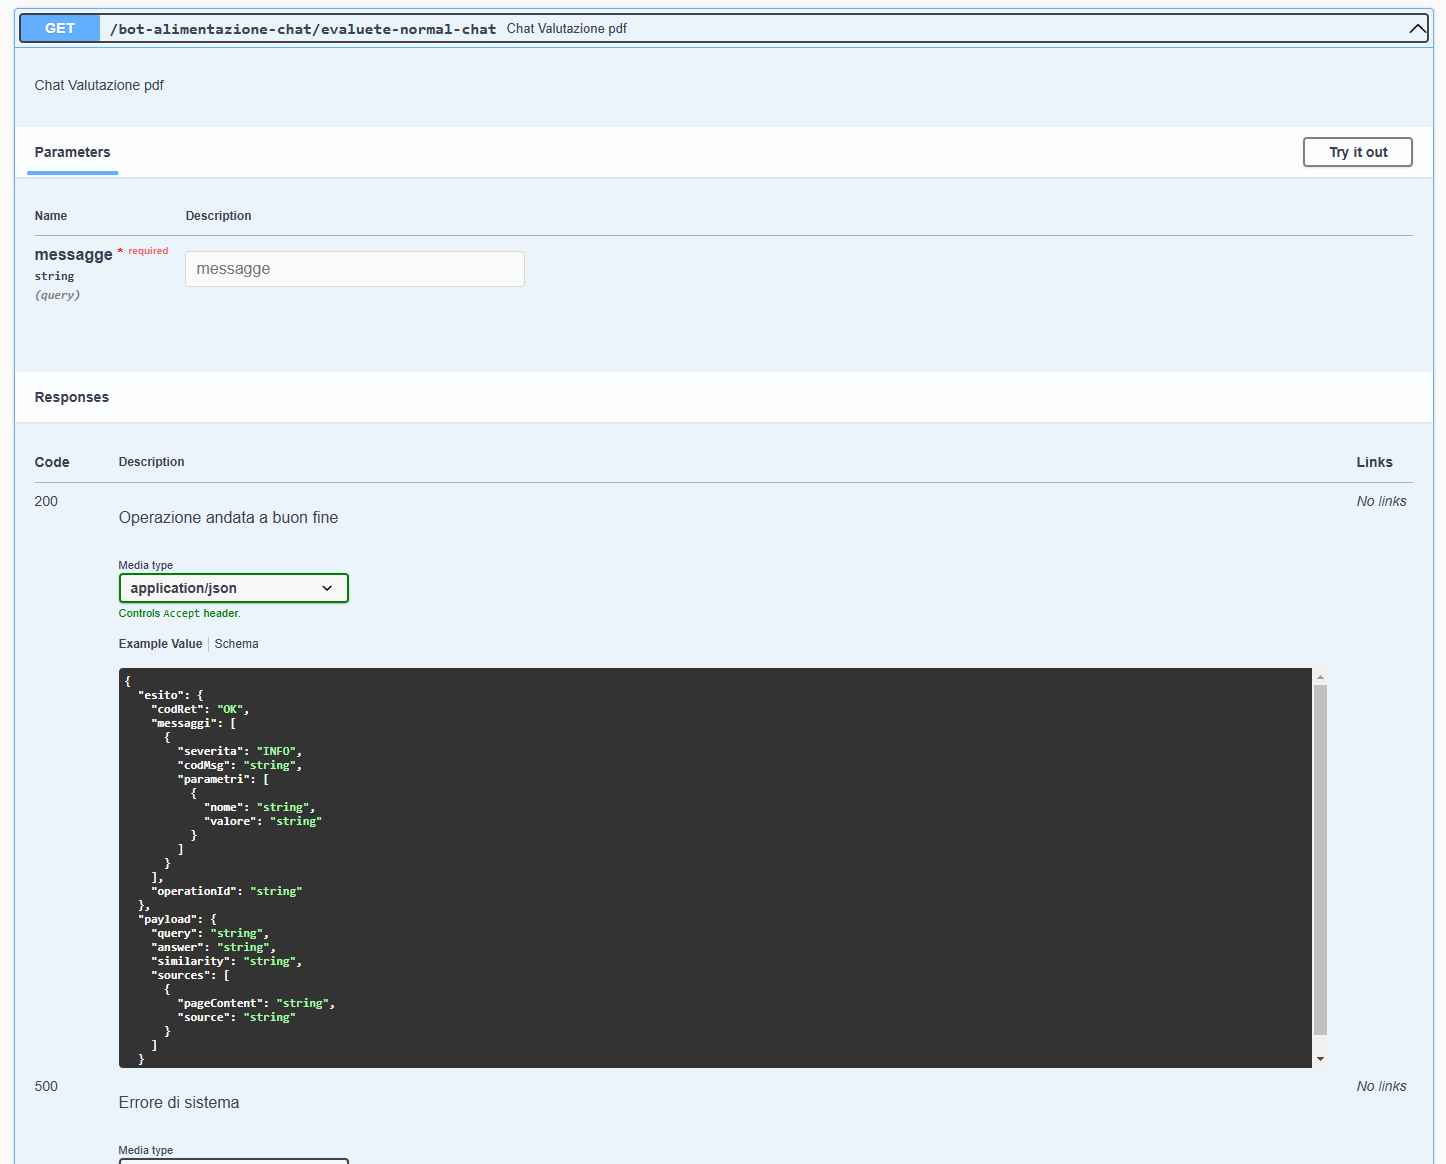
\includegraphics[width=0.9\textwidth, height=0.8\textheight, keepaspectratio]{immagini/swaggerGet.png}}

In conclusione, il Backend For Frontend (BFF) rappresenta un microservizio modulare che funge da punto centrale per l'aggregazione e l'esposizione dei vari path provenienti dai microservizi sottostanti al frontend. Questo approccio permette di personalizzare le API in base alle esigenze specifiche del frontend, garantendo una maggiore coerenza nell'interazione con i vari sistemi e semplificando la logica di integrazione.

La modularità del BFF non solo facilita la manutenibilità, ma rende anche possibile l'evoluzione continua del sistema: eventuali modifiche nei microservizi sottostanti possono essere gestite internamente senza impatti diretti sul client. Inoltre, consente di ottimizzare la sicurezza e ridurre la complessità del frontend, che può interagire con un'interfaccia consolidata e semplificata.

Questo modello si adatta particolarmente bene alle architetture a microservizi, dove la crescente frammentazione dei servizi può complicare l'esposizione diretta al client. Il BFF permette di orchestrare questi servizi in modo centralizzato e scalabile, favorendo un'interazione più efficiente e mantenendo un elevato livello di flessibilità per l'aggiunta di nuove funzionalità. Le due immagini mostrate nella sezione evidenziano chiaramente come il BFF riesca a integrare i percorsi delle richieste e a fornire risposte strutturate e uniformi, dimostrando la validità di questa soluzione nell'ambito del progetto sviluppato.

\section{Chatbot Alimentazione}

Nel contesto dell’implementazione del BFF (Backend for Frontend)

\chapter{Conclusione}
 riepilogo di tutto quello che hai fatto e commenta i risultati ottenuti in fase di sperimentazione

\bibliographystyle{plain}  
\bibliography{bibliografia}
\include{ringraziamenti}
\end{document}
